






% =========----------	[ Space left here for distraction free mode] ----------==========%









\subsection{Analysis 3: What is the effect of using Directional or Diffuse-Field Arrays?}
	\label{ana3}

		Section~\ref{ana2} revealed no significant difference between using any of the different microphone arrays apart from when it comes to a 'Sense of Space'. However the difference was only found between using the spot mic mix against mixing the spot mics with either the OCT array or the Hamasaki Cube. As both of these microphone arrays belong to different groups (OCT is used as a directional array and the Hamasaki Cube as a diffuse field array) and were not significantly different from each other, it can also be stated that the use of directional or diffuse field arrays is also not statistically significant.

		Analysing the bar chart in figure~\ref{image:sa_allmics} however it is possible to come to some conclusions about particular microphone configurations. For example, looking at the scores for Sense of Space, the three diffuse field microphone in position C whilst viewing from position A can be said to objectively perform worse than the three of the directional microphones at position A (ESMA, ORTF, ST450). However as the Eigenmke scores higher than all of them, drawing a conclusion that one microphone type is superior would be a incorrect. A more collated visualisation of overall microphone configuration performance can be seen in figure~\ref{image:sa_allmic_avgQ}, highlighting the narrow lead of the OCT microphone configuration.

		\textbf{Conclusion}
		There appears to be no significant effect of using either a directional or diffuse-field microphone array providing that spot microphones alone are not used

		\begin{figure}
			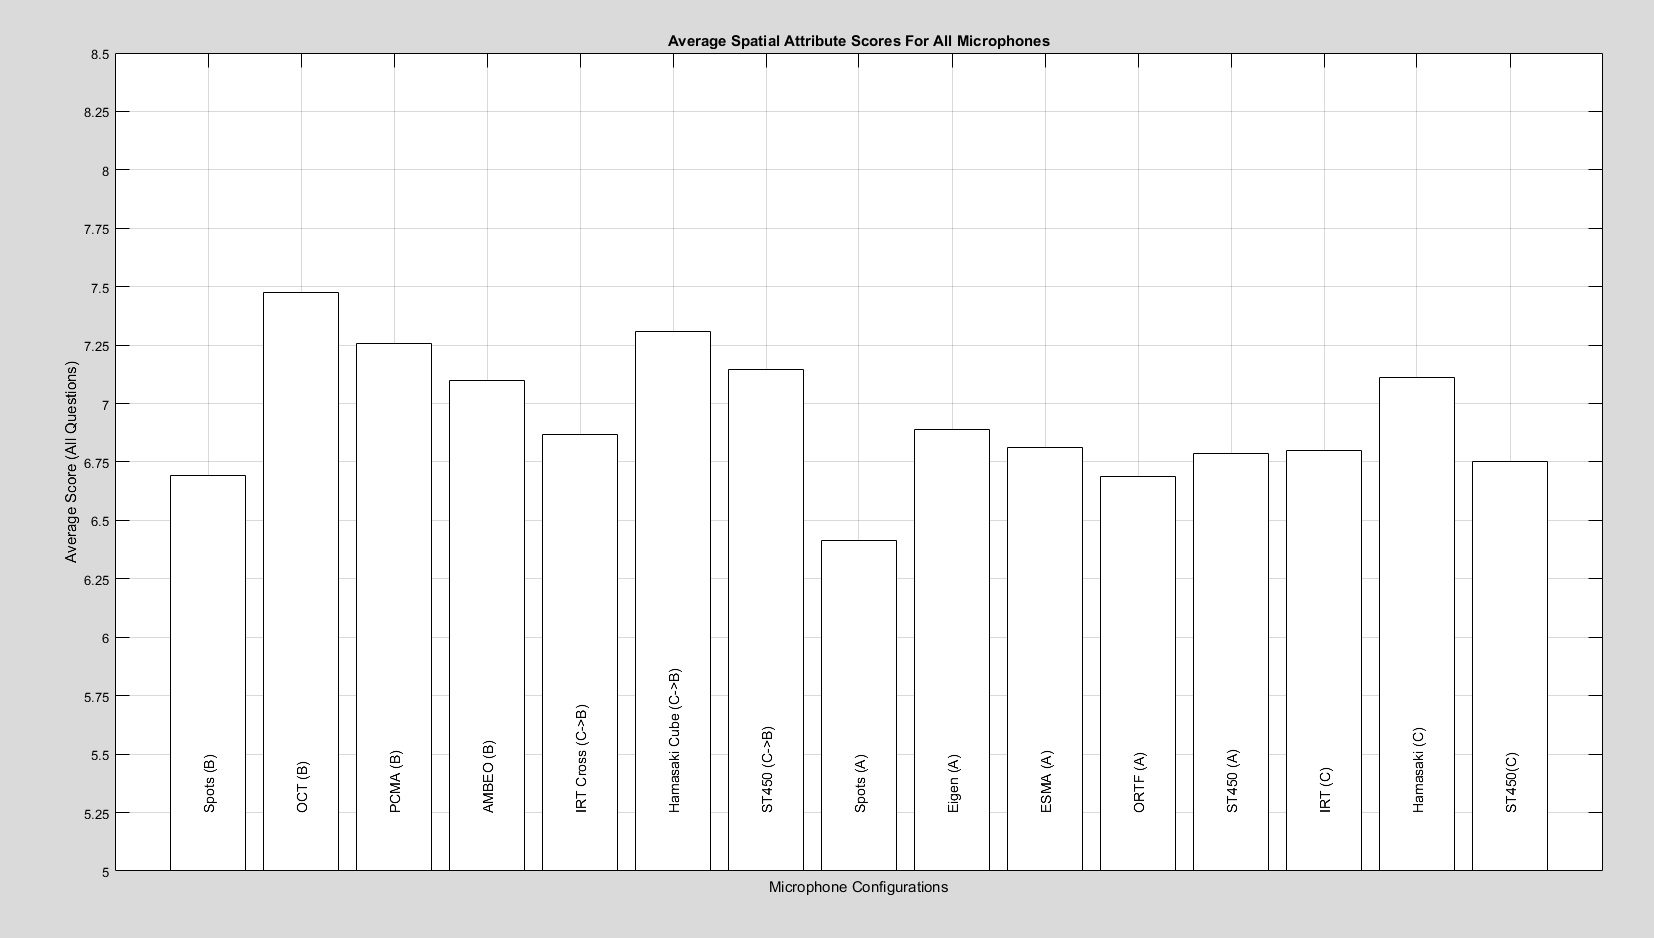
\includegraphics[width=\linewidth]{{images/plots/ana3_allmics_performance.PNG}}
			\caption{Bar chart showing the average spatial attribute score across all microphones.}
			\label{image:sa_allmic_avgQ} 
		\end{figure}		